%% Creator: Inkscape 1.3.2 (1:1.3.2+202311252150+091e20ef0f), www.inkscape.org
%% PDF/EPS/PS + LaTeX output extension by Johan Engelen, 2010
%% Accompanies image file 'Displacement_current_in_capacitor.pdf' (pdf, eps, ps)
%%
%% To include the image in your LaTeX document, write
%%   \input{<filename>.pdf_tex}
%%  instead of
%%   \includegraphics{<filename>.pdf}
%% To scale the image, write
%%   \def\svgwidth{<desired width>}
%%   \input{<filename>.pdf_tex}
%%  instead of
%%   \includegraphics[width=<desired width>]{<filename>.pdf}
%%
%% Images with a different path to the parent latex file can
%% be accessed with the `import' package (which may need to be
%% installed) using
%%   \usepackage{import}
%% in the preamble, and then including the image with
%%   \import{<path to file>}{<filename>.pdf_tex}
%% Alternatively, one can specify
%%   \graphicspath{{<path to file>/}}
%% 
%% For more information, please see info/svg-inkscape on CTAN:
%%   http://tug.ctan.org/tex-archive/info/svg-inkscape
%%
\begingroup%
  \makeatletter%
  \providecommand\color[2][]{%
    \errmessage{(Inkscape) Color is used for the text in Inkscape, but the package 'color.sty' is not loaded}%
    \renewcommand\color[2][]{}%
  }%
  \providecommand\transparent[1]{%
    \errmessage{(Inkscape) Transparency is used (non-zero) for the text in Inkscape, but the package 'transparent.sty' is not loaded}%
    \renewcommand\transparent[1]{}%
  }%
  \providecommand\rotatebox[2]{#2}%
  \newcommand*\fsize{\dimexpr\f@size pt\relax}%
  \newcommand*\lineheight[1]{\fontsize{\fsize}{#1\fsize}\selectfont}%
  \ifx\svgwidth\undefined%
    \setlength{\unitlength}{558.07086182bp}%
    \ifx\svgscale\undefined%
      \relax%
    \else%
      \setlength{\unitlength}{\unitlength * \real{\svgscale}}%
    \fi%
  \else%
    \setlength{\unitlength}{\svgwidth}%
  \fi%
  \global\let\svgwidth\undefined%
  \global\let\svgscale\undefined%
  \makeatother%
  \begin{picture}(1,1.07513228)%
  	\LARGE
    \lineheight{1}%
    \setlength\tabcolsep{0pt}%
    \put(0,0){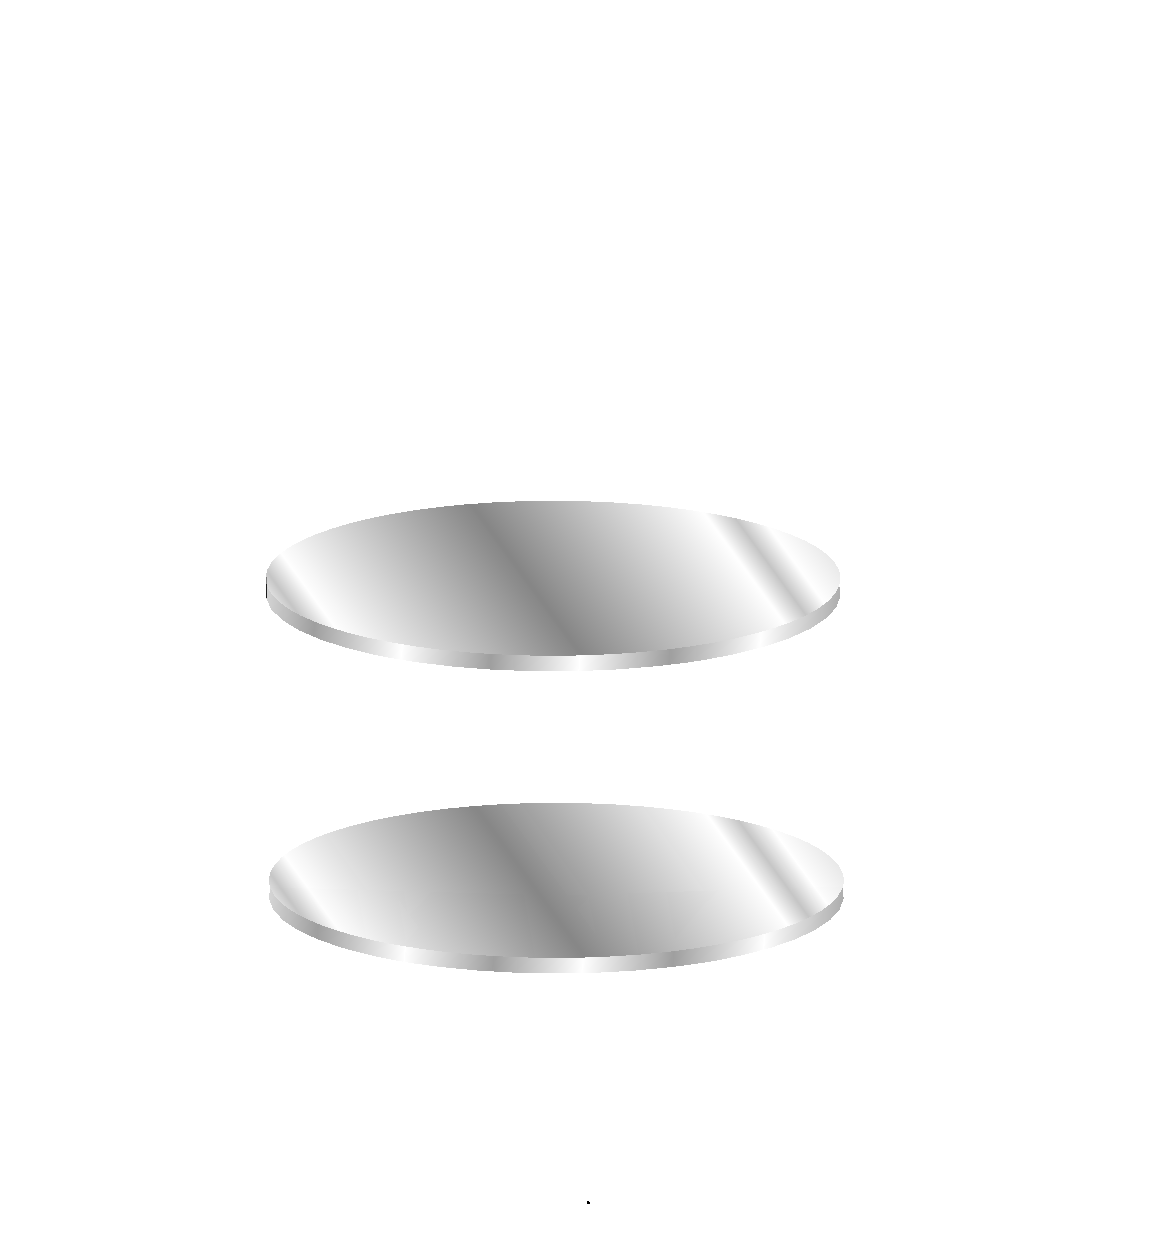
\includegraphics[width=\unitlength,page=1]{res/Displacement_current_in_capacitor.pdf}}%
    \put(0.81736302,0.77152816){\color[rgb]{0.00392157,0,0.02352941}\makebox(0,0)[lt]{\lineheight{0}\smash{\begin{tabular}[t]{l}  \end{tabular}}}}%
    \put(0.80510767,0.77557303){\color[rgb]{0.00392157,0,0.02352941}\makebox(0,0)[lt]{\lineheight{0}\smash{\begin{tabular}[t]{l}$\partial S$\end{tabular}}}}%
    \put(0.71325474,0.38769329){\color[rgb]{0.63921569,0,0}\makebox(0,0)[lt]{\lineheight{0}\smash{\begin{tabular}[t]{l} $\vec{E}$\end{tabular}}}}%
    \put(0.72489797,0.37527524){\color[rgb]{0.63921569,0,0}\makebox(0,0)[lt]{\lineheight{0}\smash{\begin{tabular}[t]{l}  \end{tabular}}}}%
    \put(0,0){\includegraphics[width=\unitlength,page=2]{res/Displacement_current_in_capacitor.pdf}}%
    \put(0.6843464,0.64225882){\color[rgb]{0,0,0}\makebox(0,0)[lt]{\lineheight{0}\smash{\begin{tabular}[t]{l}\textit{ }\end{tabular}}}}%
    \put(0.72235811,0.62596803){\color[rgb]{0,0,0}\makebox(0,0)[lt]{\lineheight{0}\smash{\begin{tabular}[t]{l}\textit{ }\end{tabular}}}}%
    \put(0,0){\includegraphics[width=\unitlength,page=3]{res/Displacement_current_in_capacitor.pdf}}%
    \put(0.36100101,0.9169215){\color[rgb]{0.00392157,0,0.02352941}\makebox(0,0)[lt]{\lineheight{0}\smash{\begin{tabular}[t]{l}$\vec{B}$\end{tabular}}}}%
    \put(0.35215045,0.88599982){\color[rgb]{0.00392157,0,0.02352941}\makebox(0,0)[lt]{\lineheight{0}\smash{\begin{tabular}[t]{l}  \end{tabular}}}}%
    \put(0.34592959,0.9042503){\color[rgb]{0.00392157,0,0.02352941}\makebox(0,0)[lt]{\lineheight{0}\smash{\begin{tabular}[t]{l}  \end{tabular}}}}%
    \put(0.50399451,0.98641512){\color[rgb]{0.00392157,0,0.02352941}\makebox(0,0)[lt]{\lineheight{0}\smash{\begin{tabular}[t]{l} $I$\end{tabular}}}}%
    \put(0.56342076,0.76035686){\color[rgb]{0.00392157,0,0.02352941}\makebox(0,0)[lt]{\lineheight{0}\smash{\begin{tabular}[t]{l}$S_1$\end{tabular}}}}%
    \put(0.70490985,0.6322398){\color[rgb]{0.00392157,0,0.02352941}\makebox(0,0)[lt]{\lineheight{0}\smash{\begin{tabular}[t]{l}$S_2$\end{tabular}}}}%
    \put(0.81445733,0.62002532){\color[rgb]{0.00392157,0,0.02352941}\makebox(0,0)[lt]{\lineheight{0}\smash{\begin{tabular}[t]{l}  \end{tabular}}}}%
    \put(0.49365715,0.07981598){\color[rgb]{0.00392157,0,0.02352941}\makebox(0,0)[lt]{\lineheight{0}\smash{\begin{tabular}[t]{l}$I$\end{tabular}}}}%
  \end{picture}%
\endgroup%
